\chapter{Verfahren zur Generierung von Mapping Daten der Umwelt}

\section{Simultaneous Localisation and Mapping}

Simultaneous Localisation and Mapping, kurz SLAM, ist ein Verfahren zum Analyse einer unbekannten Umgebung und Erstellung einer Map, während gleichzeitig die lokale Position innerhalb dieser Map bestimmt wird. Die Lösung dieses SLAM Problems war vorallem in der Robotik eine fundamentale Aufgabe der letzten zwei Jahrzehnte. Das meistern dieser Technik würde Roboter wirklich autonom steuern lassen. Bei SLAM wird die Bewegung des Objekts an sich durch den Raum und die Position aller zur positionsbestimmung notwendigen Merkmale berechnet, ohne auf vorheriges Wissen, über Position oder Lage im Raum, Kenntniss zu haben. (vgl. \cite{slam} S. 1-2)

\begin{figure}[H]
	\centering
	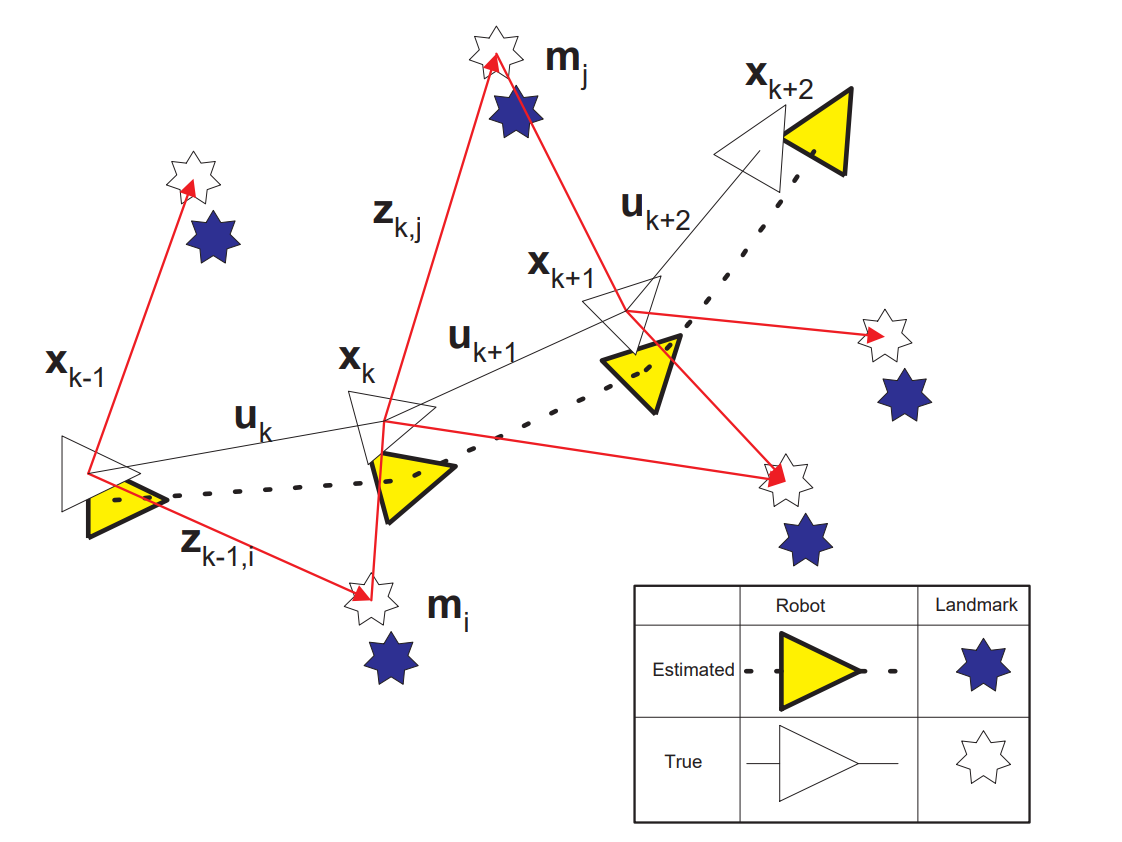
\includegraphics[scale=0.35]{slam_problem.png}
	\caption{Das SLAM Problem: Die wahren absoluten Positionen der extrahierten Features sind nie wirklich bekannt. Bildquelle \cite{slam}}
\end{figure} 

Wie in Abbildung 3.1. erkennbar ist, bewegt sich ein Roboter durch eine unbekannte Umgebung und nimmt mit seinem Sensor Features der näheren Objekte (Landmarks) auf. Wobei \large\textbf{x}\normalsize\textit{k} der Vektor des Roboters,  \large\textbf{u}\normalsize\textit{k} der Bewegungsvektor, \large\textbf{m}\normalsize\textit{i} der Vektor des Landmarks und \large\textbf{z}\normalsize\textit{ik} die Oberservation eines Landmarks durch den Roboter zur Zeit \large\textit{k }\normalsize sind. Wie man sehen kann, ist der Fehler zwischen echten und geschätzten Landmarks, bei allen geschätzten Landmarks ähnlich, was an der initialen Betrachtung der Umgebung liegt. Zu diesem Zeitpunk wird nur das erste Feature erkannt. Daraus kann man schließen, dass die Fehler in der Schätzung der Landmarkpositionen korrelieren. Praktisch bedeutet dies, dass die relative Position zweier Landmarks, \large\textbf{m}\normalsize\textit{i} - \large\textbf{m}\normalsize\textit{j} zueinander sehr genau sein kann, auch wenn die absolute Position sehr ungenau ist. 

Je mehr Landmarks in das Modell aufgenommen werden, desto gleichbleibend besser wird das Modell der relativen Positionen, egal wie sich der Roboter bewegt. Dieser Prozess wird in Abbildung 3.2. veranschaulicht.

\begin{figure}[H]
	\centering
	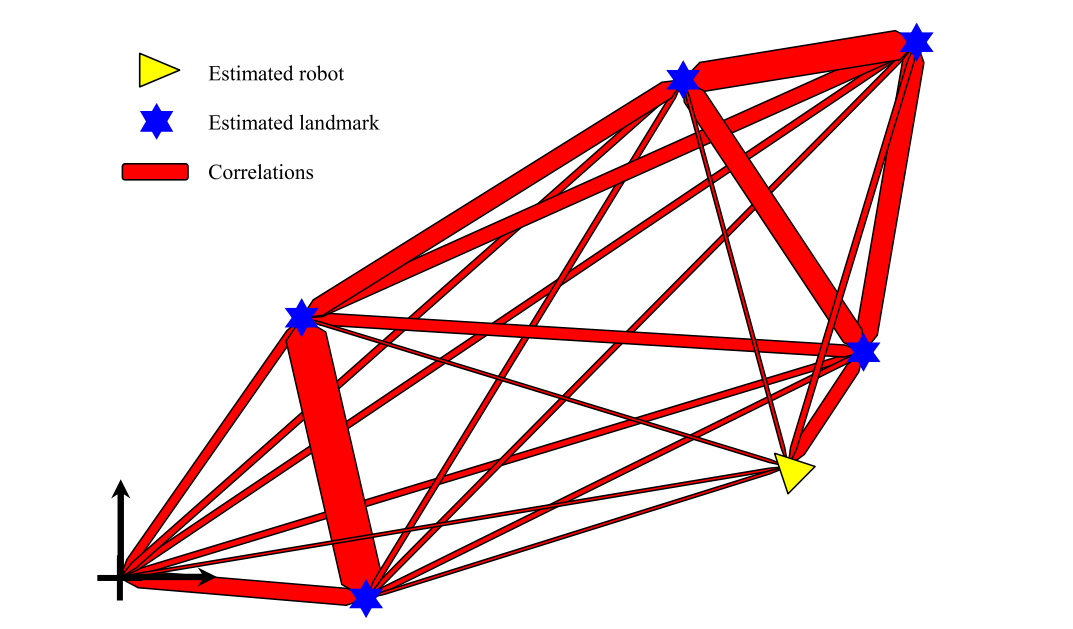
\includegraphics[scale=0.55]{slam_springs.png}
	\caption{Die Landmarks sind durch Federn verbunden, welche die Korrelation zwischen ihnen darstellen.  Bildquelle \cite{slam}}
\end{figure}  

Während sich der Roboter durch die Umgebung bewegt, werden die Korrelationen stetig aktualisiert. Je mehr Beobachtungen über die Umwelt gemacht werden, desto steifer werden die Federn in diesem Modell. Im Nachhinein werden neue Beobachtungen von Landmarks durch das ganze Netzwerk propagiert und je nach Input, kleinere oder größere Anpassungen vorgenommen.

Lösungen für das SLAM Problem benötigen eine angemessene Repräsentation für die Observierungen der Landmarks, welche eine konsistente und schnelle Berechnung ermöglichen. Die geläufigste Repräsentation besteht in der Form einer Zustandsraumdarstellung mit Gaußschen Rauschen, was zur Verwendung des \glqq Extended Kalman Filter\grqq (EKF) führt. Eine weitere alternative Repräsentation ist die Beschreibung der Features als Datenset aus Stichproben in einer nicht gaußschen Wahrscheinlichkeitsverteilung. Diese Methodik benutzt den \glqq Rao-Blackwellised particle filter\grqq oder den Fast-SLAM Algorithmus. (vgl. \cite{slam} S. 2-4)


\subsection{EKF-SLAM}

\url{http://www.iri.upc.edu/people/jsola/JoanSola/objectes/curs_SLAM/SLAM2D/SLAM%20course.pdf}

\subsection{FAST-SLAM}

\url{http://www.cs.cmu.edu/~mmde/mmdeaaai2002.pdf}
\url{http://srl.informatik.uni-freiburg.de/publicationsdir/grisettiRAS07.pdf}


\subsection{SLAM für mobiles Augumented Reality}

Das Ziel von Augumented Reality ist es virtuelle Objekte oder Informationen in die echte Welt zu integrieren, um den Benutzer zusätzliche Informationen in die betrachtete Szene zu liefern. Dazu ist es notwendig, die echte und die virtuelle Welt präzise aneinander auszurichten. Dann kann für jedes Frame aus der Sequenz des Videobildes die genaue Position des mobilen Gerätes bestimmt werden. Um dieses Ziel des exakten Matchings von Realität und generierter Virtueller Realität zu erreichen, ist "Camera Localization", also die Lokalisierung der Kamera im dreidimensionalen Raum, anhand von aufgenommenen zweidimensionalen Daten, die Schlüsseltechnologie für alle Augumented Reality Anwendungen. (vgl. \cite{slam_mobile} S.1)

\url{https://hal.inria.fr/hal-00994756/document}
\url{https://pdfs.semanticscholar.org/00f4/41387f04f40aad6491ce23bdeb0ece17d12e.pdf}



\subsection{SLAM als Core für viele AR APIs}